\section{Auswertung}
\label{sec:Auswertung}


Im folgenden werden die Theoriewerte aus \autoref{tab:literatur}, die der Literatur entnommen wurden, verwendet \cite{x_ray_database}.
Die zugehörigen Winkel jeweiliger Materialien wurden dann nach \autoref{eq:Winkel} berechnet.
Es folgt 
\begin{equation*}
  \theta = \arcsin \left( \frac{h c}{2 d E} \right)
\end{equation*}
Dabei wurde $n = 1$ gesetzt und $\lambda$ durch die bekannte Gleichung 
\begin{equation*}
  \lambda = \frac{h \cdot c}{E}
\end{equation*}
berechnet.
Weiterhin werden für die Theoriewerte der Kupferlinien
\begin{align*}
  E_{\mathrm{K}, \mathrm{abs}} &=8,987 \mathrm{keV} \, \\
  E_{\mathrm{K}, \alpha}^{\mathrm{lit}} &=8,048 \mathrm{keV} 
\end{align*}
und
\begin{equation*}
  E_{\mathrm{K}, \beta}^{\mathrm{lit}} =8,906 \mathrm{keV} \, .
\end{equation*}
angenommen \cite{x_ray_database}.
Daraus resultieren dann auch durch \autoref{eq:sigma} die $\sigma_i$'s
\begin{align*}
  \sigma_{1} &=3,29 \, ,\\
  \sigma_{2} &=12,38 \\ 
  \intertext{und}
  \sigma_{3} &=21,68 \, .
\end{align*}
 
\begin{table}
  \centering
  \caption{Theoriewerte für die Messwerte \cite{x_ray_database}.}
  \label{tab:literatur}
  \begin{tabular}{ccccc} 
    \hline Element & $Z$ & $\sigma_{\mathrm{K, Lit}}$& $E_{\mathrm{K, Lit}}$ / keV & $\theta_{\mathrm{K, Lit}}$ / ° \\
    \hline 
    $\mathrm{Zn}$ & 30 & 3,57 & 9,65   & 18,60  \\
    $\mathrm{Ga}$ & 31 & 3,60 & 10,38  & 17,25  \\
    $\mathrm{Ge}$ & 32 & 3,66 & 11,11  & 16,08  \\
    $\mathrm{Br}$ & 35 & 3,84 & 13,48  & 13,20  \\
    $\mathrm{Rb}$ & 37 & 3,94 & 15,2   & 11,68   \\
    $\mathrm{Sr}$ & 38 & 3,98 & 16,12  & 11,01  \\
    $\mathrm{Zr}$ & 40 & 4,09 & 18,0   & 9,85    \\
    \hline
  \end{tabular}
\end{table}

\subsection{Überprüfung der Bragg - Bedingung}
Zunächst soll die Bragg-Bedingung nachgewiesen werden.
Die Messwerte sind in \autoref{fig:bragg_2} aufgetragen.
Der Sollwinkel liegt bei $28°$.
Mittels Python wurde das Maximum bei $28°$ gefunden.

\begin{figure}
  \centering
  \caption{Messwerte zur Untersuchung der Bragg-Bedingung}
  \label{fig:bragg_2}
  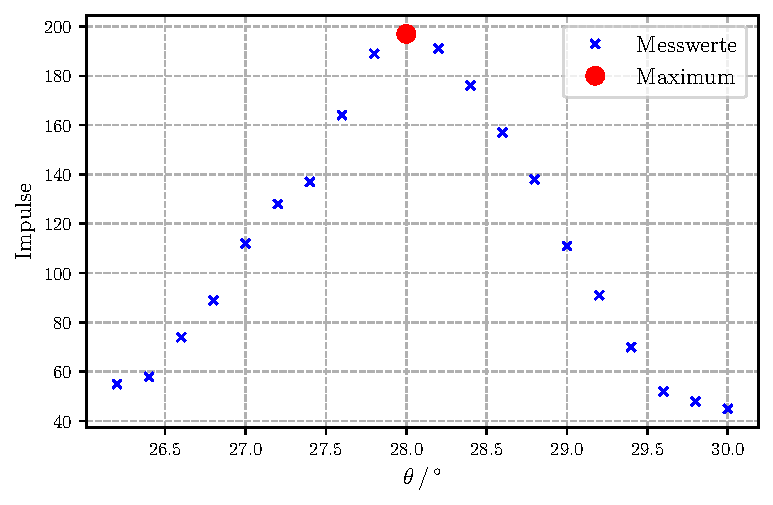
\includegraphics[width=0.5 \linewidth]{build/bragg.pdf}
\end{figure}

\subsection{Emissionsspektrum von Kupfer}
Im folgenden wird das Emissionsspektrum von Kupfer untersucht.
Aufgetragen sind die Messdaten, die über einen USB-Stick beim Versuch gespeichert und ausgelesen wurden, in \autoref{fig:kupfer1}.
Das Maximum der Bremsstrahlung wurde ebenfalls per Python bei $\qty{11.8}{°}$ ermittelt.  
Um die charakteristische Strahlung genauer zu untersuchen wird der Bereich der großen Peaks besser aufgelöst und in \autoref{fig:kupfer2} abgebildet.
Aus den Peaks lassen sich dann die Energien mit zu
\begin{align*}
  E_{\text{K}_\alpha} = \qty{8.077}{keV} &&\text{und}&& E_{\text{K}_\beta} = \qty{8.914}{keV}
\end{align*}
berechnen.
Die Halbwertsbreiten liefern die Energiedifferenzen
\begin{align*}
  \increment E_{\text{K}_\alpha} = \qty{154.5}{keV} &&\text{und}&& \increment E_{\text{K}_\beta} = \qty{195.8}{keV} \, .
\end{align*}
Für das Auflösungsvermögen gilt die Gleichung
\begin{equation*}
  A = \frac{E}{\increment E} \, ,
\end{equation*}
woraus die Werte
\begin{align*}
  A_{\text{K}_\alpha} = 41,24 && \text{und} && A_{\text{K}_\beta} = 57,69
\end{align*}
bestimmt werden.
Schließlich werden noch die Abschirmkonstanten mit \autoref{eq:sigma} bestimmt.
Hier wird für das Errechnen von $\sigma_2$ und $\sigma_3$ der theoretische Wert von $\sigma_1$ herangezogen, da sonst keine Bestimmung der anderen Möglich wäre. 
Es folgt
\begin{align*}
  \sigma_{1} &= 3,29 \, ,\\
  \sigma_{2} &= 12,62 \\ 
  \intertext{und}
  \sigma_{3} &= 21.93 \, .
\end{align*}

\begin{figure}
  \centering
  \caption{Messreihe zur Untersuchung des Emissionsspektrums von Kupfer.}
  \label{fig:kupfer1}
  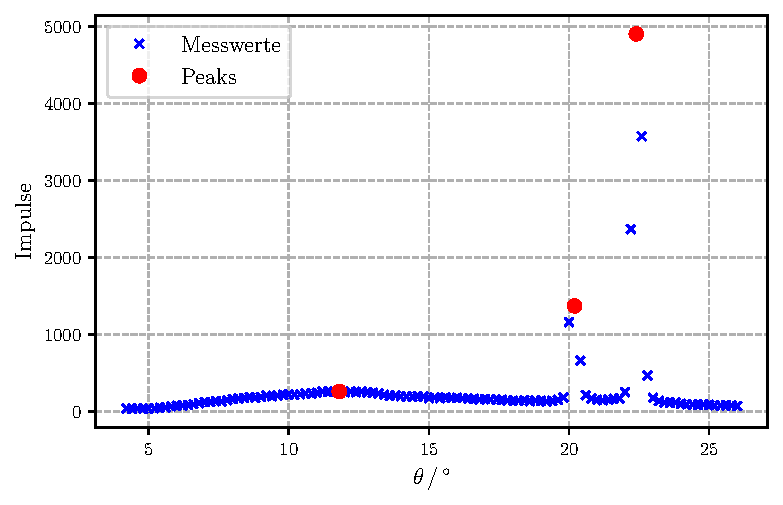
\includegraphics[width=0.5 \linewidth]{build/kupfer1.pdf}
\end{figure}

\begin{figure}
  \centering
  \caption{ Messreihe zur genaueren Untersuchung des Emissionsspektrums von Kupfer.}
  \label{fig:kupfer2}
  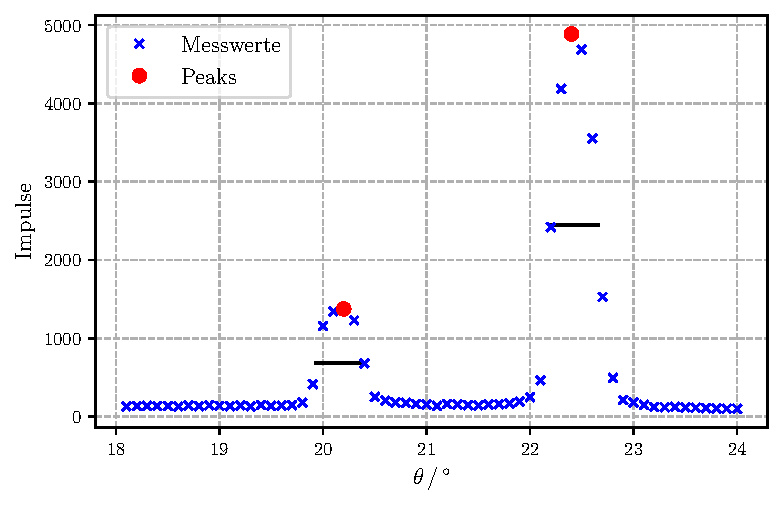
\includegraphics[width=0.5 \linewidth]{build/kupfer2.pdf}
\end{figure}

\subsection{Analyse der Absorptionsspektren}

Abschließend sollen die Absorptionsspektren verschiedenster Materialien ermittelt werden.
Hierfür wird die Zählrate $N$ der gemessenen Impulse gegen den Winkel $\theta$ aufgetragen.
Die Absorptionskante wird in den folgenden Plots eingezeichnet.
Zusätzlich wird eine vertikale Linie durch die Mitte dieser Kante gelegt.
Die Mitte ist durch die Gleichung
\begin{equation*}
  I_K = \frac{I_K^\text{min} + I_K^\text{max}}{2}
\end{equation*}
festgelegt. Dabei beschreiben $I_K^\text{min}$ und $I_K^\text{max}$ das Intensitätsminimum/- maximum der Absorptionskante.
Daraus lässt sich dann der Winkel $\theta$ bestimmen, woraus schließlich die Energie sowie die Abschirmkonstante bestimmt werden kann.
Mittels Python wird der Ansatz
\begin{equation}
  f(\theta) = \theta \cdot a + b
\end{equation}
gewählt.
Daraus lässt sich dann $\theta$ durch
\begin{equation}
  \theta = \frac{I_K - b}{a}
\end{equation}
bestimmen.
\subsubsection{Zink}
Abgebildet sind die Messdaten und die Approximation des gesuchten Winkels in \autoref{fig:zink}.
Es ergibt sich $\theta = \qty{18.538}{°}$ und $E = \qty{9.681}{keV}$.
$\sigma_K$ wird zu $\sigma_K = 3.53$ bestimmt.
Dargestellt sind die Messdaten und die Absorptionskante in \autoref{fig:zink}.
\begin{figure}[H]
  \centering
  \caption{Absorptionsspektrum von Zink.}
  \label{fig:zink}
  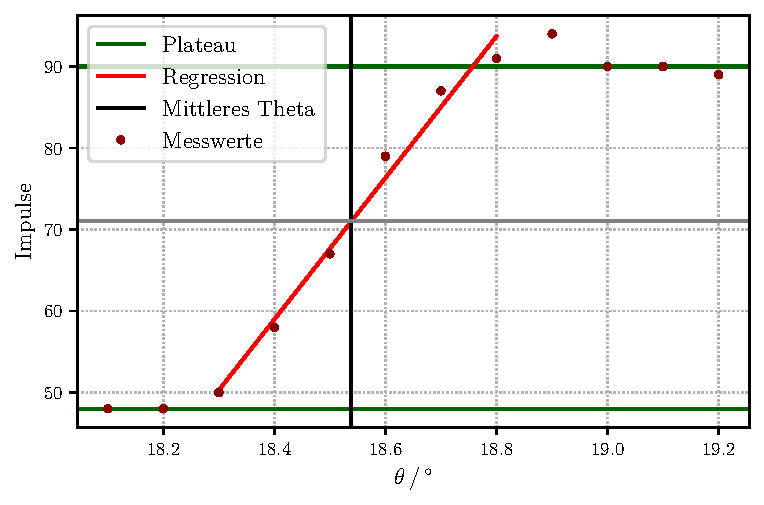
\includegraphics[width=0.5 \linewidth]{build/zink.pdf}
\end{figure}

\subsubsection{Gallium}
Dargestellt sind die Messdaten in \autoref{fig:gallium}.
Für Gallium ergibt sich eine Energie von $E = \qty{10.393}{\keV}$ für $\theta = \qty{17.23}{°}$.
$\sigma_K$ wird zu $\sigma_K = 3.56$ berechnet.
\begin{figure}[H]
  \centering
  \caption{Absorbtionsspektrum von Gallium.}
  \label{fig:gallium}
  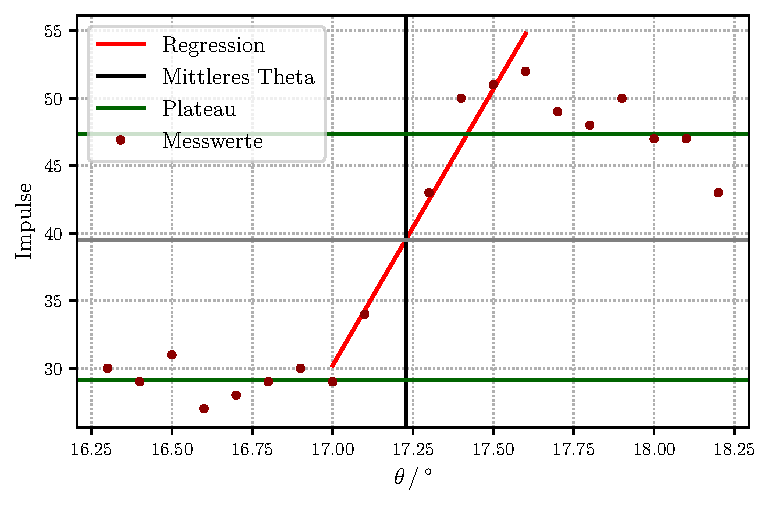
\includegraphics[width=0.5 \linewidth]{build/gallium.pdf}
\end{figure}

\subsubsection{Brom}
Dargestellt sind die Messdaten in \autoref{fig:brom}.
Für Brom ergibt sich eine Energie von $\qty{13.546}{\keV}$ für $\theta = \qty{13.13}{°}$.
$\sigma_K$ berechnet sich zu $\sigma_K = 3.76$.
\begin{figure} [H]
  \centering
  \caption{Absorbtionsspektrum von Brom.}
  \label{fig:brom}
  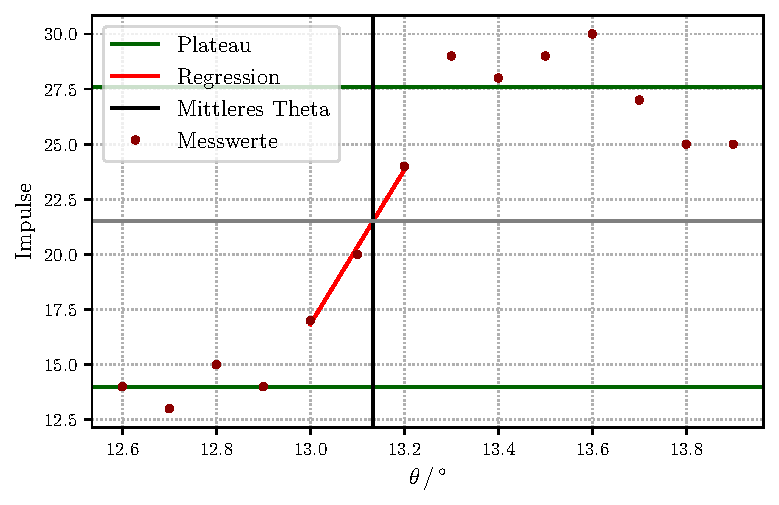
\includegraphics[width=0.5 \linewidth]{build/brom.pdf}
\end{figure}


\subsubsection{Strontium}
Für Strontium ergibt sich ein Winkel von $\qty{10.99}{°}$, woraus eine Energie von $E = \qty{16.139}{keV}$ folgt.
Dargestellt ist die Messreihe in \autoref{fig:strontium}
$\sigma_K$ wird zu $\sigma_K = 3.96$ bestimmt.
\begin{figure}[H]
  \centering
  \caption{Absorbtionsspektrum von Strontium.}
  \label{fig:strontium}
  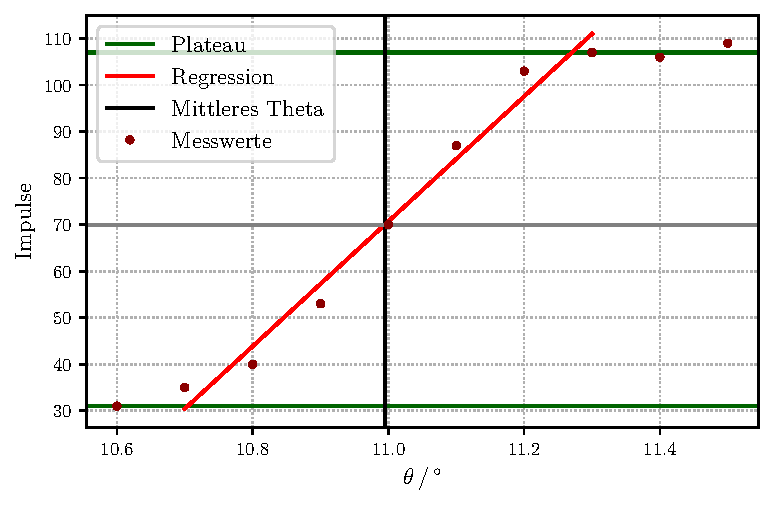
\includegraphics[width=0.5 \linewidth]{build/strontium.pdf}
\end{figure}

\subsubsection{Zirkonium}
Bei Zirkonium ergab sich nach der Ausgleichsrechnung $\theta = \qty{9.91}{°}$ und $E = \qty{17.884}{keV}$.
Die Messreihe und die Regression sind in \autoref{fig:zirkonium} dargestellt.
$\sigma_K$ wird zu $\sigma_K = 4.21$ berechnet.
\begin{figure}[H]
  \centering
  \caption{Absorbtionsspektrum von Zirkonium.}
  \label{fig:zirkonium}
  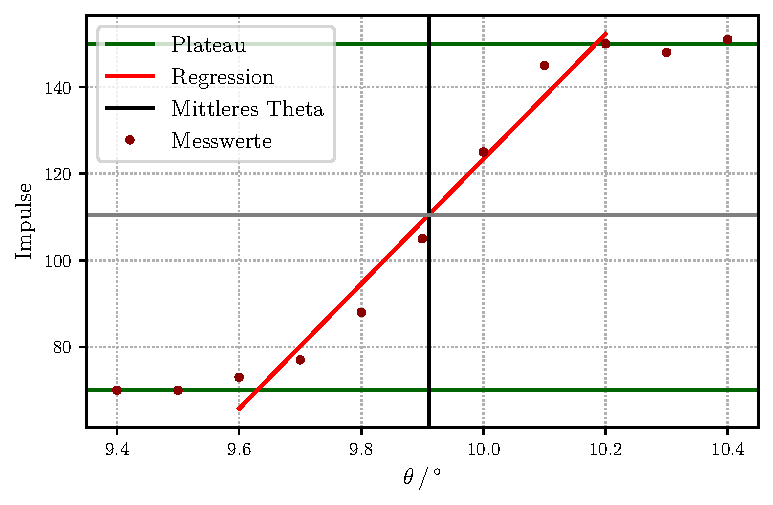
\includegraphics[width=0.5 \linewidth]{build/zirkonium.pdf}
\end{figure}

\subsection{Moseley's Gesetz}
Nun wird mit den gewonnenen Energien das Moseley'sche Gesetz verifiziert werden.
Hierfür wird der Ansatz
\begin{equation*}
  f(Z) = a \cdot Z + b
\end{equation*}
gewählt. Dabei werden die Wurzeln der ermittelten Energien gegen die zugehörigen $Z$'s aufgetragen.
Die Regression ist dargestellt in \autoref{fig:moseley}.
Aus der linearen Regression mittels Python ergeben sich die Parameter
\begin{align*}
  a = \qty{3.55(0.024)}{\eV}^{-\frac{1}{2}} && \text{und} && b  = \qty{-8.035(0.825)}{\eV}^{-\frac{1}{2}} \, .
\end{align*}
Daraus lässt sich nun die experimentell ermittelte Rydberg-Energie zu
\begin{equation*}
  E_\text{Ryd} = a^2 = \qty{12.6(0.17)}{\eV}
\end{equation*}
berechnen.

\begin{figure}
  \centering
  \caption{Regressionsgerade zur Verifizierung des Moseley'schen Gesetzes.}
  \label{fig:moseley}
  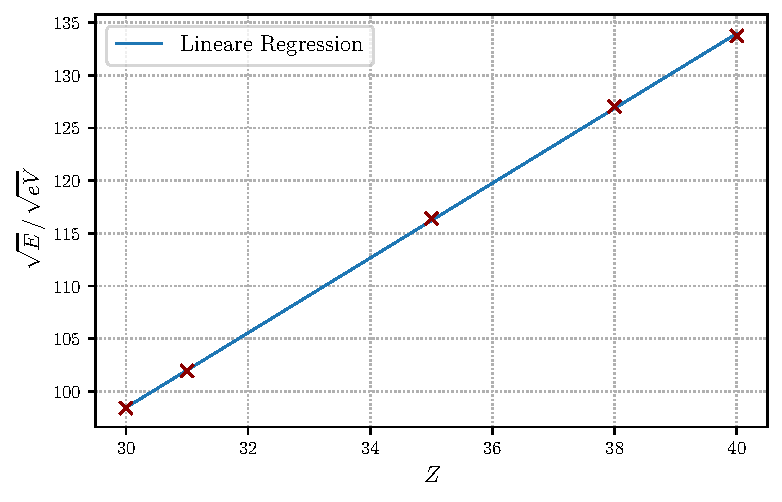
\includegraphics[width=0.5 \linewidth]{build/moseley.pdf}
\end{figure}